\documentclass{pre-tfg}

\usepackage{listings}
\usepackage{formular}
\usepackage[pdftex]{graphicx}
\usepackage{hyperref}
\usepackage{todonotes}
\usepackage{amsmath}

\showhelp  % comenta o borra para eliminar ayudas

\title{(TITLE)}
\author{María González Gutiérrez}
\docdate{(MONTH)}{2020}


\DeclareGraphicsExtensions{.pdf,.png,.jpg}

\usepackage{color}
\definecolor{gray97}{gray}{.97}
\definecolor{gray75}{gray}{.75}
\definecolor{gray45}{gray}{.45}

\lstset{ frame=Ltb,
     framerule=0pt,
     aboveskip=0.5cm,
     framextopmargin=3pt,
     framexbottommargin=3pt,
     framexleftmargin=0.4cm,
     framesep=0pt,
     rulesep=.4pt,
     backgroundcolor=\color{gray97},
     rulesepcolor=\color{black},
     %
     stringstyle=\ttfamily,
     showstringspaces = false,
     basicstyle=\small\ttfamily,
     commentstyle=\color{gray45},
     keywordstyle=\bfseries,
     %
     numbers=left,
     numbersep=15pt,
     numberstyle=\tiny,
     numberfirstline = false,
     breaklines=true,
   }

% minimizar fragmentado de listados
\lstnewenvironment{listing}[1][]
   {\lstset{#1}\pagebreak[0]}{\pagebreak[0]}

\lstdefinestyle{consola}
   {basicstyle=\scriptsize\bf\ttfamily,
    backgroundcolor=\color{gray75},
   }

\lstdefinestyle{C}
   {language=C,
   }


\renewcommand*\lstlistingname{Listado}



\begin{document}

\maketitle
\tableofcontents

\newpage


\section{INTRODUCCIÓN Y OBJETIVOS}

Empecé el proyecto porque me gusta el fanfiction y el análisis de datos, y AO3 tiene una base de datos muy grande  y accesible. Además, las comunidades de fanfic son muy activas y producen una vasta cantidad de contenido muy detallado; son básicamente una gran discusión entre los fans de una obra sobre qué es lo que dicha obra significa para ellos, y sobretodo, qué es lo que a ellos les hubiese gustado llegar a ver realizado en el texto de la misma.

En literatura comparada se suelen tener en cuenta dos perspectivas a la hora de analizar una obra: la de la teoría del autor, que tiene en cuenta lo que el autor quería comunicar y plasmar en esa obra, y la de la "muerte del autor"\cite{Barthes}, que tiene en cuenta el mensaje con el que los lectores se quedan tras leer la obra (independientemente de si coincide con el que el autor quería comunicar).
Para entender el mensaje de una obra de forma plena\cite{ellis_2018}, es necesario tener en cuenta tanto la intención comunicativa del autor, como el mensaje que al final los lectores acaban entendiendo. Y como cada lector es hijo de su padre y de su madre, acaban surgiendo muchas posibles interpretaciones distintas a partir de un único texto.

Tradicionalmente, los académicos solamente han tenido en cuenta las opiniones de un grupo reducido de personas (compuesto principalmente por otros académicos) a la hora de analizar una obra desde la perspectiva de la muerte del autor, ya que el lector común no suele tener a su disposición las herramientas necesarias para difundir sus interpretaciones. Sin embargo, desde que Internet y los foros como \textit{LiveJournal} se han vuelto accesibles a grandes partes de la población, miles de comunidades fan empezaron a organizarse justamente con la intención de poner en común sus interpretaciones, de expresar sus críticas y opiniones. No todas estas discusiones tienen lugar en forma de fanfiction, pero es un género muy popular en las comunidades fans, y yo personalmente estoy muy familiarizada con sus estructuras y códigos.

Estas comunidades de Internet están generando una cantidad inmensa de opiniones y perspectivas en torno a un tema común en foros públicamente accesibles, y me pareció interesante la idea de crear un sistema que sea capaz de recoger y procesar toda esta información para crear un "abanico" de las distintas interpretaciones que existen en una comunidad fan, especialmente aquellas sobre los personajes y las relaciones entre ellos. El resultado final se podría utilizar como herramienta dentro de la propia comunidad fan, para observar cómo tienden a interpretar a ciertos personajes a nivel de comunidad y cómo estas interpretaciones cambian a lo largo del tiempo, o en distintas subsecciones dentro de la comunidad en general. También se podría utilizar como herramienta general de análisis literario, aplicándola primero a la obra original y luego a un conjunto de fanfics representativos, y observando cuáles son las diferencias entre la perspectiva del autor original y la de los lectores (convertidos en autores fan).

Al empezar el proyecto, no sabía mucho sobre análisis de texto, por lo que empecé a estudiar sobre análisis de texto natural y extracción de información usando el libro \textit{Natural Language Processing} (Jacob Eisenstein, MIT Press). Tras la fase de recogida y limpieza de datos (explicado en detalle en las secciones \ref{sec:recogidadatos} y \ref{sec:limpiezadatos}), el proceso de extracción de información que tenía que seguir consistía en:


\begin{enumerate}
	\item Identificación de entidades
	\item Identificación de relaciones entre entidades
	\item Identificación de eventos
\end{enumerate}

%Sin embargo, otra parte importante del proyecto iba a consistir en la extracción y selección de textos de Internet, organizarlos de alguna forma y procesarlos para que sean comprensibles para los algoritmos de análisis de texto. Éste proceso está explicado en detalle en las secciones \ref{sec:recogidadatos} y \ref{sec:limpiezadatos}.


\section{FANFICTION Y ARCHIVE OF OUR OWN}

Fanfiction (del inglés \textit{fan fiction}, 'ficción del fan', y abreviado como 'fanfic') es el nombre que recibe un texto basado en una historia ya existente (normalmente con copyright), en particular cuando el autor es fan de la obra de la cual su texto deriva. Son, por lo tanto, textos de ficción sin ánimo de lucro que los fans escriben como expresión de su creatividad.

El concepto detrás del fanfiction es, en esencia, una ausencia percibida en la historia original. Uno se termina un libro o un videojuego y siente que le falta algo: el pasado de un protagonista, una perspectiva distinta de un conflicto, una relación que acabó o nunca empezó, qué sucede después del final, o quizás que a la historia le hacían falta doscientas páginas más, o incluso que tendría que haber sido de un género literario distinto... Hay algo en la historia que está ausente. El lector se queda con ganas de explorar más a fondo el mundo y los personajes que el autor ha creado, y de aquí nace el impulso de crear historias propias en las que se exploran dichas ausencias. Por tanto, no es sorprendente descubrir que hay muchos fanfics en los que se cambia el destino de tal o cuál personaje, que exploran qué sucede tras el final, o que llevan a cabo exploraciones exhaustivas de los conflictos, los personajes y sus motivaciones desde perspectivas distintas a las de la obra original.

Todos estos motivos hacen que el fanfiction se considere una obra derivada\cite{woosh_1998}, y está en su naturaleza el reflejar las opiniones y críticas que el autor tiene de la obra original: qué es lo que le gusta, qué temas siente que faltan en la obra, qué cosas tendrían que haberse explicado desde una perspectiva distinta, etc.

Por ejemplo, es evidente al leer los libros de la saga \textit{Harry Potter} que el texto quiere que pienses que Ron Weasly, el mejor amigo del protagonista, es un chico un poco torpe y bocazas pero con buen corazón, y un buen amigo de Harry. Sin embargo, muchos fans no interpretaron a Ron como torpe y bocazas, sino como egocéntrico e insensible, y hay no pocos fanfics en los que Ron y Harry discuten y dejan de ser amigos, o en los que Ron es directamente un villano aliado con Voldemort.

Cuando los fans de una misma obra se reúnen y organizan, se crean comunidades fan llamadas "fandoms", que suelen crear foros donde intercambiar sus impresiones, teorías y, por supuesto, fanfiction y otras formas de arte fan. Es evidente que existe un intercambio de ideas en foros de discusión y otras comunidades online explícitamente creadas para conversar, pero ya que es totalmente posible inferir las opiniones de un autor a partir de sus fanfics, tanto escribir como leer fanfiction son actividades que contribuyen al discurso general del fandom, ayudando a popularizar algunas teorías y generando las suyas propias.

Cuando un fandom alcanza un cierto nivel de madurez, algunas teorías se consolidan y el fandom acaba formando, a nivel de comunidad, una interpretación propia de la obra original. Para distinguir la perspectiva del fandom de la que realmente pretende transmitir la obra original, en los fandoms se distingue entre el \textit{fanom} y el canon. Siguiendo el ejemplo de \textit{Harry Potter}, el Ron Weasly del \textit{fanon} es una persona egoísta que sólo es amigo de Harry por interés, mientras que el Ron Weasly del canon tiene una amistad sincera con Harry. \textit{Fanon}, por tanto, es el 'conjunto de teorías basadas en el material original que, aunque generalmente parecen ser la interpretación 'obvia' o 'única' de los hechos canónicos, no son realmente parte del canon'\cite{uncanny_2017}.


%Ésta es sólo una de las formas de escribir fanfic que hay. Existen muchos fanfics que cambian la historia original de formas mucho más radicales, explorando cómo hubiese sido Star Wars si Luke Skywalker hubiese caído al lado oscuro, o cómo actuarían los personajes de Juego de Tronos si fuesen trabajadores normales en una cafetería de Toronto, por poner algunos ejemplos. El fan convertido en autor puede añadir o quitar a la historia original lo que considere oportuno para contar su propia visión personal.

En resumen, las comunidades fan tienen una interpretación propia de la obra original llamada \textit{"fanon"}, que influencia los fanfics que los miembros de dicha comunidad van a escribir y, a su vez, los escritores de fanfic también crean y popularizan interpretaciones que se acaban convirtiendo en parte del \textit{fanon}.

Como se ve en el ejemplo de \textit{Harry Potter}, las relaciones entre personajes son una de las mayores fuentes de especulación entre los fans, especialmente las relaciones románticas. En general, los personajes a los cuales los fans les tienen manía acaban convertidos en villanos (o, como mínimo, enemigo de los protagonistas) en los fanfics, incluso aunque en la obra original sean aliados. Naturalmente, lo mismo sucede a la inversa: los fans tienden a convertir en amigos y aliados a los personajes que les gustan, incluso aunque en la obra original sean los villanos de la historia. Por tanto, simplemente contrastando las relaciones presentes en un fanfic con las relaciones de la obra original podemos tener una buena idea de cuál es la interpretación del autor del fanfic.

Las relaciones románticas entre personajes son una parte enorme de la especulación fan. El romance es uno de los temas más populares, y aunque las relaciones canónicas atraen naturalmente la atención de muchos fans, 'inventar' parejas en el \textit{fanon} no sólo es común, sino una de las principales actividades de un fandom. Los fans ven parejas y conflictos amorosos tanto entre amigos como enemigos, \todo{continuar parejas y fandom}Un villano que es muy popular entre los fans tiene garantizado que tendrá fanfic en los que cambia de bando, convirtiéndose en aliado y pareja del protagonista (no necesariamente en ese orden).

\missingfigure{fig: grafos de relaciones entre personajes de un fanfic y mismos personajes en la obra original. Harry Potter?}

No todas las parejas son igual de populares en el fandom, sino que por lo general hay una o dos, como mucho tres parejas que monopolizan la atención y creatividad de los fans, y la popular de cada una suele ser independiente de si la pareja es canon o no en el material original.

En términos legales y de derechos de autor, la mayoría de legislaciones considera el fanfiction como un tipo de obra derivada \cite{woosh_1998} y por tanto entra dentro del \textit{fair use}. A día de hoy, la mayoría de fanfics se publican en sitios web de toda índole, destacando entre ellos \href{archiveofourown.org}{Archive Of Our Own}, que es un archivo open-source y sin ánimo de lucro creado expresamente para alojar obras creadas por fans. Según sus datos de mayo de 2020, tiene más de dos millones de usuarios registrados y más de seis millones de trabajos alojados. 


En particular elegí descargar los fanfics basados en \textit{Good Omens}, un libro de Terry Pratchett y Neil Gaiman, tanto por la cantidad de relatos existente como por mi familiaridad con esa comunidad.

Además de la cantidad y variedad de relatos que aloja, los motivos por el que elegí extraer los datos de \todo[size=\small]{por qué escogí AO3 sobre FF.net y Wattpad} Archive Of Our Own son su herramienta de búsqueda y filtrado, su sistema de etiquetas y el hecho de que permite descargar el archivo en HTML. Archive Of Our Own permite filtrar fanfics según varios parámetros y genera un enlace a ese subconjunto de relatos particular, muy útil para descargar una gran cantidad de datos.

\section{INTELIGENCIA ARTIFICIAL Y ANÁLISIS DE TEXTO}
Lorem ipsum dolor sit amet \todo[size=\tiny]{mirar intro del libro de eisenstein}

consectetur adipiscing elit \todo[size=\tiny]{explicar bag of words + función que calcula peso en función de vector características}
%El procesado de textos en lenguaje natural es una de las preocupaciones de la inteligencia artificial, y del aprendizaje automático en particular. 

%Otras aplicaciones similares a la mía: resumir texto?
% ontología star trek: \href{https://pr-owl.org/basics/ontostartrek.php}{ontología star trek}




\section{RECOGIDA Y LIMPIEZA DE DATOS}

\subsection{CREANDO UN SCRAPER PARA ARCHIVE OF OUR OWN}
\label{sec:recogidadatos}

En el momento en el que decidí utilizar los fanfics de \textit{Good Omens} para el proyecto, dicho libro tenía unos 22000 fanfics en \href{archiveofourown.org}{Archive Of Our Own} (AO3 para abreviar). Sin embargo, de todos esos relatos sólo me interesaban los que están en inglés y los que realmente contuvieran texto (puesto que, aunque AO3 se centra en texto, permite todo tipo de archivos multimedia), de modo que utilicé el sistema de filtrado del sitio para seleccionar sólo los fanfics en inglés y que no estuvieran etiquetadas como "fanart", "podfic", etc, ya que indican que la obra no tiene texto. Tras este filtrado, quedaron 20190 relatos. \todo{literaturizar esta sección}

AO3 crea un enlace que lleva siempre a ese subconjunto de relatos, al cual puedo enviar peticiones HTTP GET y navegar las páginas. Cada página contiene un máximo de 20 fanfics, y antes de descargarlos es necesario llevar a cabo un segundo filtrado para evitar las obras sin texto que no hayan sido etiquetadas como tal por su autor. Decidí crear dos \textit{scrapers} distintos, uno para navegar por las páginas, filtrar y guardar los \textit{links} en un archivo, y otro que simplemente lee dicho archivo y realiza descargas.

\begin{itemize}
	\item El primer \textit{scraper} envía peticiones a AO3, explora el HTML de cada página para encontrar los objetos que encapsulan la información de cada fanfic, selecciona aquellos que tengan al menos 40 palabras por capítulo y crea una lista con los enlaces, que guarda en un archivo \textit{txt}.
	\item El segundo \textit{scraper} recorre los enlaces de dicho archivo y los descarga en una carpeta del sistema. Está hecho de tal manera que se le puede indicar qué tramo de la lista tiene que descargar (por ejemplo, del número 5000 al 6000).
	
\end{itemize}

Ambos \textit{scrapers} se encontraban de vez en cuando con el error 429 (Too Many Requests) y el 404 (Page Not Found). Se capturan fácilmente con un \textit{try-catch} que detecta el status de la página; para el 429 simplemente lanza una espera de dos minutos tras la cual reanuda su ejecución por donde la dejó, y para el 404 simplemente pasa a la siguiente, pues este error indica que el autor ha borrado su obra de la página y ya no está accesible.
 
Decidí dividir este proceso en dos programas (el de navegación y filtrado, y el que únicamente descarga) en vez de hacerlo todo en uno porque descargar los más de 20000 archivos de una vez lógicamente tardaría varias horas, y pensé que sería más pragmático si ejecuto una vez el \textit{scraper} crea una lista de enlaces, y luego ya ejecuto todas las veces que sean necesarias el \textit{scraper} que descarga, descargando cada vez un tramo distinto de la lista. De esta forma, pude descargar todos los fanfics en grupos de 2000 (alrededor de una hora y media), pudiendo tener el ordenador libre el resto del tiempo.

El poder ejecutar varias veces el segundo \textit{scraper} sin tener que volver a empezar desde el principio también demostró ser útil para lidiar con errores de red.

Ambos \textit{scrapers} utilizan la librería bs4 y BeautifulSoup para descargar y manejar los archivos HTTP. El resultado de su ejecución es una carpeta con 818,8 MB de archivos HTML

\subsection{LIMPIEZA DE DATOS}
\label{sec:limpiezadatos}
Los fanfics descargados en HTML vienen con metadatos relacionados con la historia, el autor y cuándo fueron publicados, entre otros. Además, la mayoría de fanfics tienen notas del autor, comentarios y sinopsis que, aunque forman parte del cuerpo del texto, no son relevantes para el análisis que voy a realizar.
Me interesa poder recuperar fácilmente los metadatos útiles de cada fanfic, además de convertirlo a texto plano eliminando todos los metadatos y los comentarios del autor, por lo que decidí reunir todas estas funciones en dos clases, FanficCleaner y FanficHTMLHandler, encapsuladas en un programa fanfic\_util.py

\begin{itemize}
	\item FanficCleaner tiene métodos para extraer el cuerpo del texto de un archivo HTML, sin metadatos, comentarios ni notas del autor. También tiene la función de guardar el texto en un archivo txt en un \textit{path} a elegir.
	\item FanficHTMLHandler tiene métodos que permiten extraer metadatos del archivo HTML de un fanfic, como por ejemplo los personajes principales, el número de capítulos y su clasificación.
\end{itemize}

Debido a que los archivos HTML están organizados en carpetas, utilizo listas con sus \textit{path} para identificarlos y acceder a ellos. Los métodos de FanficCleaner y FanficHTML reciben tramos de estas listas para acceder y manejar los archivos deseados.
Para ello, el programa utiliza las librerías BeautifulSoup y html2text.

\section {EXTRACCIÓN DE DATOS A PARTIR DE TEXTO}
\todo[size=\tiny]{Explicar los programas que hice para familiarizarme con NLTK}

\subsection{ALGORITMO DE IDENTIFICACIÓN DE ENTIDADES}

En la identificación de entidades, se considera una entidad a los personajes, los lugares y las instituciones, entre otras cosas, que haya sido nombrada en el texto. Un algoritmo capaz de identificar entidades nombradas tiene que poder dividir un texto en tramos y asignarle una etiqueta de entidad ("Persona", "País", etc) a cada uno. Esta tarea además requiere que las palabras del texto hayan sido previamente etiquetadas con su rol morfológico.

Por estos motivos, la librería NLTK parecía la más idónea para la tarea. Es una librería de python que contiene herramientas básicas para el análisis de texto, y en particular me interesaba que venía con un \textit{part of speech tagger} (es decir, un identificador de rol morfológico) ya programado y entrenado. NLTK también viene con un identificador de entidades ya entrenado, pero quería programar uno que fuera más preciso y adaptado a mi conjunto de datos.

Además del identificador de rol morfológico, NLTK también tiene una clase llamada \textit{ChunkParser} cuyo trabajo es dividir un texto en tramos. Todas las funciones de la librería que se encargan de dividir y/o etiquetar texto (como el identificador de rol morfológico) heredan de alguna versión de la clase \textit{ChunkParser}, de modo que la idea para el algoritmo era modificar la clase \textit{ChunkParserI} para convertirla en un identificador de secuencias basado en características.
\todo[size=\small]{citar ref al sitio web en cuyo código me he basado}

Un identificador de secuencias basado en características trata de asignar un peso a un tramo concreto, y según el peso, le asigna una etiqueta u otra. Este peso se calcula como una función de las características del propio tramo, así como de los tramos que le preceden.
El programador puede elegir las características que considere más importantes, pero hay algunas que son bien conocidas como las más importantes para reconocer entidades, como:

\begin{itemize}
	\item El rol morfológico de la palabra actual, las anteriores y las siguientes.
	\item La forma de la palabra, las anteriores y las siguientes (si empiezan por mayúscula, si tienen signos de puntuación, si son siglas, etc)
	\item Los prefijos y/o sufijos de la palabra actual, las anteriores  y las siguientes.
	\item Si la palabra anterior ha sido identificada como una entidad o no.
	
\end{itemize}

El conjunto de características de cada tramo se llama vector de características, y se utiliza para calcular un "peso" que se corresponde con la probabilidad de que un tramo X con un vector de características V tenga una etiqueta Y. El algoritmo al final asigna a cada tramo la etiqueta cuyo peso sea el más alto.

El cómo se calcula exactamente ese peso depende del modelo matemático a utilizar. A la versión modificada de ChunkParserI para la identificación de entidades la llame NERChunker (NER por Named Entitiy Recognition), y tiene tres versiones:

\begin{itemize}
	\item NERChunkerv1 y NERChunkerv3 utilizan un modelo de regresión logística (también llamado modelo de entropía máxima), a través de la clase MaxentClassifier de NLTK. Para que NLTK pueda utilizar esta clase correctamente, es necesario tener instalado el módulo Megam para python, que no viene incluído en NLTK. La única diferencia entre la versión 1 y la 3 de este chunker es que la 3 maneja las estructuras de NLTK para oraciones y etiquetas de forma ligeramente más rápida.
	\item NERChunkerv2, que utiliza un modelo de naïve Bayes a través de la clase ClassifierBasedTagger de NLTK.
	
\end{itemize}

Las versiones \textit{v1} y \textit{v3} de \textit{NERChunker} obtuvieron los mejores resultados en la evaluación, y la \textit{v3} es algo más rápida, por lo que es la versión definitiva del identificador de entidades. Todas estas versiones, junto con sus funciones auxiliares, se encuentran encapsuladas en el archivo \textit{NERChunkers.py}, para ser utilizadas donde se las necesite.

\missingfigure{fig: evaluaciones de las versiones de NERChunker y el NER de NLTK}

Puesto que tanto los clasificadores de regresión logística como los de \textit{naïve} Bayes son algoritmos de aprendizaje supervisado, antes de poder utilizar (o evaluar) cualquiera de las versiones de \textit{NERChunker} era necesario entrenarlas con un conjunto de datos ya etiquetados. El problema aquí es que NLTK, a pesar de incluir un corpus muy extenso en la propia librería, sólo tiene dos conjuntos de datos para identificación de entidades: uno en español y el otro en holandés. Todos los textos a analizar en el proyecto están en inglés, obligándome a buscar un conjunto ajeno a NLTK y finalmente decidiéndome por \textit{Groningen Meaning Bank} (GMB). GMB es un \textit{dataset} para identificación de entidades específicamente en inglés, grande, con una gran variedad de etiquetas de entidad y, sobretodo, con un formato de etiquetado sencillo de entender,cosa importante puesto que al ser ajeno a NLTK, GMB utiliza etiquetas distintas que son necesario adaptar para que \textit{MaxentClassifier} pueda trabajar con ellas.

GMB utiliza la notación IOB para etiquetar entidades, y separa cada palabra de la siguiente por un carácter de nueva línea, y cada frase, por dos. De modo que la frase \textit{"Mr. Blair left for Turkey Friday from Brussels."} en GMB tendrá el aspecto de la \ref{fig:tags1}

\begin{figure}[h]
	\label{fig:tags1}
	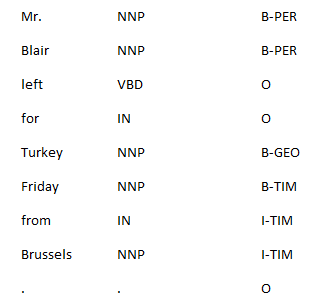
\includegraphics[scale=0.9]{GMB_tag}
	\caption{Frase etiquetada por GMB. De izquierda a derecha, las columnas representan la palabra a etiquetar, la etiqueta de rol morfológico, y la etiqueta IOB.}
	\centering
\end{figure}

Cuando el programa detecta una entidad de tipo persona, etiqueta como 'B-PER' la primera palabra de la secuencia, mientras que el resto de palabras dentro de la secuencia son etiquetadas como 'I-PER'. Similarmente, si la entidad es de tipo geográfico las etiquetas usadas serán 'B-GEO' y 'I-GEO', si es de tiempo serán 'B-TIM' y 'I-TIM', etc. Si una palabra no forma parte de ninguna secuencia de entidad, se etiqueta como 'O'.

NLTK, por su parte, no utiliza la notación IOB  ni caracteres de nueva línea, sino que utiliza una estructura de datos propia de tipo árbol que encapsula cada palabra y cada tramo con su etiqueta. La misma frase etiquetada por NTLK tiene el aspecto de la \ref{fig:tags2}

\begin{figure}[h]
	\label{fig:tags2}
	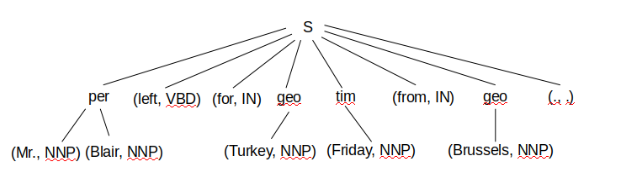
\includegraphics[scale=0.8]{NLTK_tag}
	\caption{Frase etiquetada por NLTK. Las etiquetas de entidad se encuentran en los nodos, encontrándose todas las palabras pertenecientes a una secuencia de entidad en la profundidad 2 del árbol. Las palabras que no pertenecen a ninguna secuencia de entidad se encuentran en la profundidad 1. Cada hoja del árbol contiene una tupla formada por la palabra y su etiqueta de rol morfológico.}
	\centering
\end{figure}

Como se ve, en vez de usar etiquetas IOB, NLTK organiza las palabras y su etiquetas en una estructura de árbol. La raíz, S, indica el inicio de la frase (Sentence), y las etiquetas de entidad son nodos.

En horizontal queda así:

(S, [(per, [(‘Mr.’, NNP), (‘Blair’, NNP)]), (‘left’, VBD), (‘for’, IN), (geo, [(‘Turkey’, NNP)]), (tim, [(‘Friday’, NNP)]), (‘from’, IN), (geo, [(‘Brussels’, NNP)]), (‘.’,.)])

Fue más o menos a estas alturas del proyecto cuando decidí separar el proceso de entrenar el identificador de entidades y el de utilizarlo para etiquetar texto nuevo en dos programas distintos (NERTrainer y NERTagger, respectivamente). Acceder a los textos de GMB y transformar sus etiquetas a un formato que NLTK pueda entender y acceder a los textos de la base de datos de fanfics y preprocesarlos para su posterior etiquetado mediante el programa ya entrenado han resultado serdos procesos muy distintos, y dividirlo parecía la mejor manera de tener un código limpio y claro.

\todo[size=\tiny]{listar en alguna parte las librerías: BeautifulSoup, pandas}

%%% DETALLES TÉCNICOS %%%
% POS\_tagger.py: para poder etiquetar las entidades nombradas es necesario etiquetar cada palabra con su rol morfológico, de modo que este programa se encarga de abrir los archivos html, pasarlos a texto y ponerle sus etiquetas morfológicas. Para ello utiliza los métodos de NLTK word\_tokenize y sent\_tokenize para dividir cada texto en frases y palabras, y pos\_tag para usar el clasificador por defecto de python para asignar etiquetar morfológicas en inglés. Almacena el resultado en un csv, de modo que en vez de tener preparar el archivo html y etiquetarlo cada vez que quiera identificar entidades, sólo tengo que etiquetar cada archivo una vez.
% NER\_trainer.py: entrena el algoritmo identificador de entidades usando el dataset de entrenamiento (descargado de aquí) y guarda el objeto en un archivo binario usando la librería pickle. Una vez entrenado, evalúa la precisión del algoritmo y la imprime por pantalla. Como el dataset no es parte del corpus nativo de NLTK, mucho de éste programa consiste en abrir el csv del dataset y empaquetar sus datos en listas y tuplas que sean compatibles con NLTK, y dividir el resultado en un dataset de entrenamiento y dos para hacer test (80\%, 10\% y 10\% del dataset original, respectivamente). Este programa utliza un objeto de la clase NERChunkerv1, que se encuentra en el archivo NER\_chunker.py, que se explica más abajo.
% NER\_tagger.py: utliza la libraría pickle para deserializar el archivo binario entrenado por NER\_trainer.py, y lo utiliza para etiquetar entidades nombradas en frases (usando etiquetas IOB). Utiliza el archivo csv creado por POS\_tagger para saltarse la parte de asignar etiquetas morfológicas, y guarda sus etiquetas en otro csv, de modo que gran parte de su código se dedica a lidiar con abrir, leer y actualizar archivos csv.


%En NERChunkerv1 he utilizado una interfaz de NLTK llamada ChunkParserI. Tiene el constructor y dos métodos:
%\begin{itemize}
%	\item el constructor recibe el dataset en forma de frases etiquetadas y entrena el algoritmo. El dataset que he utilizado venía con etiquetas IOB en forma de tuplas, pero NLTK usa las etiquetas IOB en otro formato, de modo que el constructor se dedica principalmente a manipular las tuplas y aplicarles el método tree2conlltags para que NLTK las entienda. Y después llama a NERTagger y le pasa el dataset ya preparado para entrenar un clasficador.
%	\item parse, que es el método que recibe una frase con etiquetas morfológicas y la etiqueta, con el clasificador ya entrenado. Devuelve la frase etiquetada con etiquetas IOB en forma de árbol, que es el formato de etiqueta que NLTK utiliza.
%	\item evaluate, que evalúa la precisión del algoritmo. Uso el de laIdentificación de eventos superclase, así que en mi código no está definido.
%\end{itemize}


%NERTagger mantiene un historial de etiquetas IOB (una lista) y depende de feature\_function, una función que recoge ciertas características (featureset) de una palabra y las devuelve en forma de diccionario. Las características que recoge son éstas:


\subsection{ALGORITMO DE IDENTIFICACIÓN DE RELACIONES}

Para este algoritmo decidí crear un algoritmo LDA, que es un algoritmo de aprendizaje no supervisado que se utiliza típicamente en identificación de temas. Para entrenar este algoritmo, seleccioné un conjunto de fanfics que sirviesen de modelo para la relación que quería que aprendiera a detectar. Por ejemplo, para entrenar un modelo LDA que detecte situaciones sexuales, preparé un conjunto de fanfics de un único capítulo en los que sucedía sexo, excluyendo otros que tenían escenas sexuales pero eran sólo una pequeña parte de una historia más larga. 

Para buscar el modelo LDA más eficiente, creé tres modelos que tenían en cuenta diferentes categorías morfológicas. Primero utilizaba el \textit{tagger} de NLTK para identificar categorías morfológicas, y el algoritmo sólo tenía en cuenta aquellas que resultaran relevantes.

\begin{itemize}
	\item El modelo B tenía en cuenta sustantivos, adverbios y verbos.
	\item El modelo C tenía en cuenta sustantivos, adjetivos y verbos.
	\item El modelo D tenía en cuenta sustantivos, adverbios, adjetivos y verbos.
\end{itemize}

Además de utilizar distintas categorías morfológicas, también probé distintos tamaños para el set de entrenamiento, de modo que cada modelo tiene dos versiones: una entrenada con 5000 fanfics y otra entrenada con 10000.

Para la evaluación de los modelos, simplemente los puse a clasificar textos nuevos, contando la cantidad de aciertos de cada uno y calculando el \textit{hit ratio} de cada uno. Los resultados aparecen en la primera tabla de la figura \ref{table:topic_evaluation}.

\begin{gather*}
hit\_ratio = \frac{correct\_guesses}{total\_number\_of\_guesses}
\end{gather*}

\begin{figure}
	\caption{Porcentaje de aciertos de cada modelo. Cada prueba se realizó tres veces.}
	\label{table:topic_evaluation}
	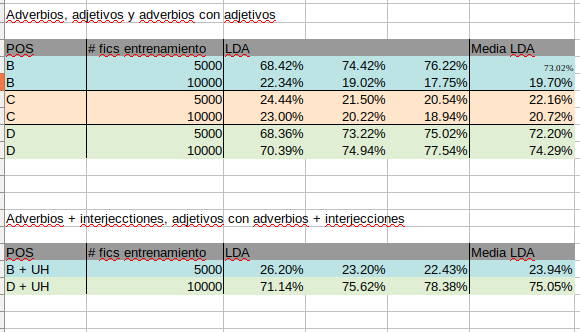
\includegraphics[scale=0.6]{topic_evaluate_table_v2}
	\centering
\end{figure}

Las primeras pruebas mostraron que los modelos B y D eran los que arrojaban mejores resultados. Observando qué otras categorías morfológicas el \textit{tagger} de NLTK puede identificar, pensé que añadir interjecciones a los modelos podría aumentar su precisión. Llamé B+UH y D+UH a los modelos resultantes, y repetí las pruebas. Los resultados están en la segunda tabla de la figura \ref{table:topic_evaluation}.

Curiosamente, el modelo D fue mejorado ligeramente teniendo en cuenta las interjecciones, pero el modelo B empeoró considerablemente.

\section{EVALUACIÓN DEL SISTEMA}


\section{REFERENCIAS}




\bibliographystyle{alpha}
\singlespacing
%\bibliography{ejemplo}
\bibliography{bib_tfg}


\end{document}


% Local Variables:
% coding: utf-8
% mode: flyspell
% ispell-local-dictionary: "castellano8"
% mode: latex
% End:
